% LAB 1: An Introduction to Linux and Python
% 
% CSE/IT 107: Introduction to Programming
% New Mexico Tech
%
% Prepared by Cynthia Veitch, William Kwan, Scott Chadde, Kaley Goatcher,
% Russell White, and Christopher Koch
% Spring 2015

% Instructional goals of this lab:
% - basic Linux command line use
% - start learning how to read the documentation (man pages, python docs)
% - Python as a calculator
% - Canvas use

\documentclass[11pt]{cselabheader}

%%%%%%%%%%%%%%%%%% SET TITLES %%%%%%%%%%%%%%%%%%%%%%%%%
\fancyhead[R]{Lab 1: An Introduction to Linux and Python}
\title{And Now for Something Completely Different\\
  {\large An Introduction to Linux and Python}}

\begin{document}

\pagenumbering{roman}
\maketitle

\hrule

\begin{quotation}
  ``Programs must be written for people to read, and only incidentally for
  machines to execute.''
\end{quotation}
\begin{flushright}
--- H. Abelson and G. Sussman (\textit{Structure and Interpretation of Computer
Programs})
\end{flushright}

\begin{quotation}
``Avoid the Gates of Hell. Use Linux.''
\end{quotation}
\begin{flushright}
--- Unknown
\end{flushright}

\begin{quotation}
``I choose to believe what I was programmed to believe.''
\end{quotation}
\begin{flushright}
  --- Robot Villager \#2 (\textit{Futurama})
\end{flushright}

\hrule
%%%%%%%%%%%%%%%%%%%%%%%%%%%%%%%%%%%%%%%%%%%%%%%%%%%%%%%%%%%%%%%%%%%%%%%%%%%
%%%%%%%%%%%%%%%%%%%%%%%%%%%%%%%%%%%%%%%%%%%%%%%%%%%%%%%%%%%%%%%%%%%%%%%%%%%
\section{Introduction}

The purpose of this lab is to introduce you to the Python programming
environment. In this lab, you will learn how to
\begin{enumerate*}
  \item log into a computer of the Tech Computer Center (ITC),
  \item learn how to use and navigate Linux,
  \item learn to use Python as an interpreter,
  \item edit and run a few short Python programs
  \item learn the basics of Python flow control, and
  \item create a tarball and submit it to Canvas.
\end{enumerate*}

Throughout this semester's labs, we will be using specially formatted text to
aid in your understanding. For example,

\begin{bashcode}
$ text in a console font within a gray box
\end{bashcode}

is text that either appears in the terminal or is to be typed into the terminal
verbatim. Even the case is important, so be sure to keep it the same! If a \$ is
used that indicates the terminal prompt. You do not type the \$.

\begin{python3code}
Text that appears in console font within a framed box is sample Python code
or program output.
\end{python3code}

\begin{pyconcode}
>>> # Text that appears in console font wihtin a framed box and is preceded by
>>> # three greater-than signs contains sample Python interpreter input.
\end{pyconcode}

Text in a \texttt{simple console font}, without a frame or background, indicates
the name of a file, a function, or some action you need to perform.

%%%%%%%%%%%%%%%%%%%%%%%%%%%%%%%%%%%%%%%%%%%%%%%%%%%%%%%%%%%%%%%%%%%%%%%%%%%
%%%%%%%%%%%%%%%%%%%%%%%%%%%%%%%%%%%%%%%%%%%%%%%%%%%%%%%%%%%%%%%%%%%%%%%%%%%
% \section{Requirements}

% In order to receive full credit for this lab, you must do the following:
% \begin{enumerate*}
% \item Log into Linux at the ITC using your assigned username.
% \item Replace the conversion constant in \texttt{sample\_c\_file.c}.
% \item Compile and run \texttt{sample\_c\_file.c}, saving the output in a script file.
% \item Add a header to the script.
% \item Edit the script file to include answers to the questions posed in this lab.
% \item Create a Tar archive of your lab submission and submit it to the lab email address.
% \end{enumerate*}

\pagebreak

\tableofcontents

\pagebreak

%%%%%%%%%%%%%%%%%%%%%%%%%%%%%%%%%%%%%%%%%%%%%%%%%%%%%%%%%%%%%%%%%%%%%%%%%%%
%%%%%%%%%%%%%%%%%%%%%%%%%%%%%%%%%%%%%%%%%%%%%%%%%%%%%%%%%%%%%%%%%%%%%%%%%%%
\pagenumbering{arabic}
\section{Linux Environment}
\label{sec:linux}

The following instructions will guide you through the Linux introduction.
Because this is an introductory lab, the instructions are rather detailed and
specific. However, it is important that you understand the concepts behind the
actions you take -- you will be repeating them throughout the semester. If you
have any questions, ask the instructor, teaching assistant, or lab assistant.

\subsection{Log in}
To log into a ITC machine, you must use your ITC username and password. If you
do not have a ITC account, you must visit the ITC office (Speare 5) to have one
activated.

If your computer is currently booted with Windows, restart it and select Fedora
(a variety of Linux) as your operating system. Please note that using Linux is a
\emph{requirement} for this lab.

\subsection{Open a Terminal}
In Linux, you will perform most actions from the command line. In order to do
this, you must first open a terminal. There are many methods for opening a
terminal; the following is just one.

% TODO: REVISE REVISE REVISE they use cinnamon now
\begin{enumerate}
  \item Click on the \texttt{Menu} button at the bottom left of the screen.
  \item In the text box that pops up as part of the menu, type in
    \texttt{Terminal} and hit return.
\end{enumerate}


\subsection{Shell}
At the terminal prompt you are using what is called a shell. A shell
provides a means to interact with the operating system. The shell also provides
the command line for you: a means to type in commands and receive feedback from
the operating system, shell, or program behind that command.

\subsubsection{Terminal Prompt}

When you open the shell, you will probably see something like this:

\begin{minted}[fontsize=\small,
  mathescape,linenos,numbersep=5pt,framesep=2mm,frame=lines,bgcolor=lightgray]{shell-session}
[username@machinename ~]$ youcantypehere
\end{minted}

This is where you type commands. We will be shortening this prompt to just a
single \$ to denote a terminal prompt for the rest of this semester's labs.

\subsection{File Hierarchy}

Unix has a logical file system, which means as an end user you don't care about
the actual physical layout and can focus on navigating the file system.

Key: Everything begins at the root directory
\texttt{/} and all other directories are children of the root directory. The
file system forms a tree.

A path consists of the names of directories and is a way to navigate from the
root file system to the desired directory. If you include the root directory in
the path this is called an absolute path. Another way to navigate the tree is to
use relative paths, which navigate the tree based on where you currently are.

An absolute path starts at the root directory \texttt{/} and gives an absolute
description of which directory or file you are refering to. For example,
\texttt{/u/ckoch/cse107/lab1/} refers to the directory as seen in the file tree
below. A relative path always references your current directory. When you are in
a shell, you always have a \textit{current working directory} from which the
relative path will go. A relative path leaves off the first \texttt{/} and uses
\texttt{..} to refer to the parent of the current working directory and
\texttt{.} to refer to the current working directory. For example, if my current
directory is \texttt{/u/ckoch/cse107/}, then \texttt{lab1} refers to the absolute
path \texttt{/u/ckoch/cse107/lab1/}, while \texttt{../} refers to the absolute
path \texttt{/u/ckoch/}, and \texttt{../../tcecil} refers to the absolute path
\texttt{/u/tcecil/}.

For example, this is a typical file system tree close to what the ITC has with
absolute file paths shown on the right:
\tikzstyle{every node}=[draw=black,thick,anchor=west]
\tikzstyle{selected}=[draw=red,fill=red!30]
\tikzstyle{optional}=[dashed,fill=gray!50]

\begin{tikzpicture}[
grow via three points={one child at (0.5,-0.7) and
two children at (0.5,-0.7) and (0.5,-1.4)},
edge from parent path={(\tikzparentnode.south) |- (\tikzchildnode.west)}]
\node {/}
child { node [label={[xshift=4.5cm, yshift=-0.58cm] /bin}] {bin} }
child { node [label={[xshift=4.5cm, yshift=-0.58cm] /dev}] {dev} }
child { node [label={[xshift=4.5cm, yshift=-0.58cm] /tmp}] {tmp} }
child { node [label={[xshift=4.5cm, yshift=-0.58cm] /u}] {u}
child { node [label={[xshift=3.95cm, yshift=-0.58cm] /u/ckoch}] {ckoch} 
  child { node [label={[xshift=3.4cm, yshift=-0.58cm] /u/ckoch/cse107}] {cse107}
    child { node [label={[xshift=2.85cm, yshift=-0.58cm] /u/ckoch/cse107/lab1}] {lab1} }
  }
}
child [missing] {}
child [missing] {}
child { node [label={[xshift=3.95cm, yshift=-0.58cm] /u/tcecil}] {tcecil}}
child { node [label={[xshift=3.95cm, yshift=-0.58cm]
/u/yourusername},optional] {yourusername}}
}
child [missing] {}
child [missing] {}
child [missing] {}
child [missing] {}
child [missing] {}
child { node [label={[xshift=4.5cm, yshift=-0.58cm] /usr}] {usr}
child { node [label={[xshift=3.95cm, yshift=-0.58cm] /usr/bin}] {bin} }
}
child [missing] {}
;
\end{tikzpicture}

\subsection{Commands}

All commands that you execute in a shell are structured in the following way:

\begin{bashcode}
$ commandname -options arguments
\end{bashcode}

Remember that the \$ just denotes a terminal prompt.

There can be any number of options and arguments, separated by spaces. For
example, if the command is \texttt{python3} and you want it to run the file
\texttt{hello.py} and you want to enter interactive mode after the file is run,
you would type

\begin{bashcode}
$ python3 -i hello.py
\end{bashcode}

in your shell. Options and arguments vary by the specific command. (Do not
worry, we will explain what python3 and the file and interactive mode mean
later.)

\subsubsection{pwd -- \textbf{P}rint \textbf{W}orking \textbf{D}irectory}

\textbf{p}rint \textbf{w}orking \textbf{d}irectory displays the
directory you are in.

\begin{bashcode}
$ pwd
/home/cse
\end{bashcode}

The directory you are currently in is called your ``working'' directory.

\subsubsection{cd -- Change Directory}
\texttt{cd} allows you to change your working directory to another location.

Syntax:

\begin{bashcode}
$ cd <path_name>
\end{bashcode}

% where the $<$path\_name$>$ is either relative or absolute.
% They don't know what that means.

\begin{bashcode}
$ cd /usr/local/bin
$ pwd
/usr/local/bin
$ cd -
\end{bashcode}

Where are you?

\begin{bashcode}
$ cd -
\end{bashcode}

Now where are you? The command \texttt{cd -} returns you to your previous
working directory.

The \texttt{-} is called a command line argument or option. To view
the list of options for a command, use the manual.

\begin{bashcode}
$ man cd
\end{bashcode}

\texttt{man} is short for manual.

To move up one directory (one node) level use dot-dot:

\begin{bashcode}
$ cd ..
\end{bashcode}

Where are you?

To move up two levels use dot-dot slash dot-dot:

\begin{bashcode}
$ cd ../..
\end{bashcode}

To go to your home directory you can type

\begin{bashcode}
$ cd /u/<user>
\end{bashcode}

where $<$user$>$ is your user name. Alternatively, use a tilde

\begin{bashcode}
$ cd ~
\end{bashcode}

or you can use

\begin{bashcode}
$ cd $HOME
\end{bashcode}

where \$HOME is an environment variable that stores the path to your
home directory. This is more useful in shell scripting than path
navigation. Use tilde instead.

Even easier than all these options is to just type \texttt{cd} without any
options. This always takes you to your home directory.

\begin{bashcode}
$ cd
\end{bashcode}

% orphaned table
See Table~\ref{tab:cd} for a summary of the arguments to \texttt{cd}.

\begin{table}[!ht]
  \centering
  \begin{tabular}{ll}
    \toprule
      \bfseries Argument & \bfseries Meaning\\
    \midrule
      <path>    & change directory to the <path> supplied \\
      ..        & change directory to parent directory \\
      $\sim$    & change directory to home directory \\
      -         & change directory to previous working directory \\
      \$HOME    & change directory to home directory \\
      {[}no argument{]} & change directory to home directory \\
    \bottomrule
  \end{tabular}
  \caption{Some possible arguments to \texttt{cd}}
  \label{tab:cd}
\end{table}

\subsubsection{man -- Manual}

To view the documentation for any command, use

\begin{bashcode}
$ man commandname
\end{bashcode}

For example,

\begin{bashcode}
$ man cd
\end{bashcode}

will show the documentation for the \texttt{cd} command. A man page will usually
include a \textit{synopsis} that tells you all the possible options and usages
of the command followed by a detailed \textit{description}, which is followed by
a section that explains all the \textit{options}. There can be many other
sections in a man page, but most man pages will have at least these three.

Please try to make use of man pages before you ask for help -- our first
suggestion regarding anything that involves Linux commands will be for you to
use the man page.

\subsubsection{ls -- Listing the Contents of a Directory}
\texttt{ls} allows you to list the contents of a directory: the files and
directories that are located there.

\begin{bashcode}
$ cd
$ ls
<a list of file names and directories contained 
with your working directory, which is currently
your home directory>
\end{bashcode}

Adding some command-line options let you see other file information:

\begin{bashcode}
$ ls -alFh 
...
-rwxr-x---.  1 scott scott  1.0K Jan 12 14:56 down_and_out*
drwxr-xr-x.  5 scott scott  4.0K Jan 21 17:04 Downloads/
-rw-r-x---.  1 scott scott  2.2K Jan 12 11:31 .emacs
...
\end{bashcode}

The \texttt{a} option shows hidden files (a.k.a. dot-files), the \texttt{l}
option produces a long listing format of file names and directories, the
\texttt{F} option adds a \texttt{*} to the end of the file if is an executable
and a \texttt{/} if it is a directory, and the \texttt{h} option prints out the
size of the file in human readable format.

Under Linux, any file whose name begins with a dot is a ``hidden'' file. Most
commands that list files in some way will hide files that begin with a dot.

\paragraph*{Understanding the Long Format Output} \hfill

The \texttt{-l} option of \texttt{ls} tells you quite a bit about a file. For a
detailed explanation of the output, please see Table 3-2 on page 16 of
\textit{The Linux Command Line} (\url{http://linuxcommand.org}).

\paragraph*{Finding More Information} \hfill

How can you see more command line options for \texttt{ls}? What is the option to
sort by file size?


\subsubsection{mkdir -- Creating Directories}
Directories are very important for organizing your work, and you should get in
the habit of creating a new directory for every lab this semester. 

To create a directory, use the \bashinline{mkdir} command as such:

\begin{bashcode}
$ mkdir directorypath
\end{bashcode}

For example, if you are in your home directory \texttt{/u/username}, you can
create the directory \texttt{cse107} in two ways: 

\begin{description}
  \item[Absolute path] \hfill

    \begin{bashcode}
$ mkdir /u/username/cse107
    \end{bashcode}

  \item[Relative path] \hfill

    \begin{bashcode}
$ mkdir cse107
    \end{bashcode}
\end{description}

%\begin{enumerate}
%\item In the terminal, change your current working directory to your home
%  directory by typing the following command:
%
%\begin{bashcode}
%$ cd
%\end{bashcode}
%
%\item Create a \texttt{cse107} directory by typing the following command;
%
%\begin{bashcode}
%$ mkdir cse107
%\end{bashcode}
%
%\item Change your current working directory to the \texttt{cse107} directory by
%  typing the following command:
%
%\begin{bashcode}
%$ cd cse107
%\end{bashcode}
%
%\item Create a subdirectory for this lab in your \texttt{cse107} directory by
%  typing the following command:
%
%\begin{bashcode}
%$ mkdir lab1
%\end{bashcode}
%
%\item Change your current working directory to the \texttt{lab1} directory by
%  typing the following command:
%
%\begin{bashcode}
%$ cd lab1
%\end{bashcode}
%
%\end{enumerate}

\begin{infobox}{Habits}
  It's a good idea to have a directory for each lab inside a directory for the
  class. For example:

\begin{tikzpicture}[
grow via three points={one child at (0.5,-0.7) and
two children at (0.5,-0.7) and (0.5,-1.4)},
edge from parent path={(\tikzparentnode.south) |- (\tikzchildnode.west)}]
\node {/}
child { node [label={[xshift=4.5cm, yshift=-0.58cm] /u}] {u}
child { node [label={[xshift=3.95cm, yshift=-0.58cm] /u/ckoch}] {ckoch} 
  child { node [label={[xshift=3.4cm, yshift=-0.58cm] /u/ckoch/cse107}] {cse107}
    child { node [label={[xshift=2.85cm, yshift=-0.58cm] /u/ckoch/cse107/lab1}] {lab1} }
    child { node [label={[xshift=2.85cm, yshift=-0.58cm] /u/ckoch/cse107/lab2}] {lab2} }
    child { node [label={[xshift=2.85cm, yshift=-0.58cm] /u/ckoch/cse107/lab3}] {lab3} }
  }
}
}
child [missing] {}
child [missing] {}
child [missing] {}
child [missing] {}
child [missing] {}
child [missing] {}
;
\end{tikzpicture}
\end{infobox}

\subsection{The Linux Command Line}

Chapters 1 through 4 of \textit{The Linux Command Line} by William Shotts cover
the above material in much more depth. The book is available online as a PDF.
Please read chapters 1 through 4 before lab 2! (This will also be announced as
the pre-lab for lab 2.)
\begin{center}
  \url{http://linuxcommand.org/tlcl.php}
\end{center}

\subsubsection{Other Commands}

To learn about these commands, please use man pages or \textit{The Linux Command
Line}.

\begin{bashcode}
cp
mv
rm
touch
cat
less
\end{bashcode}

\subsection{Start Python}

In the shell, type \texttt{python3}. It is important that you not use
\texttt{python}, but \texttt{python3}! It should look something like this:

\begin{bashcode}
$ python3
Python 3.3.2 (default, Jun 30 2014, 12:45:18) 
[GCC 4.8.2 20131212 (Red Hat 4.8.2-7)] on linux
Type "help", "copyright", "credits" or "license" for more information.
>>> 
\end{bashcode}

\subsection{Summary}
\label{sec:linux.res}

Commands to know for future labs:
\begin{multicols}{3}
\begin{itemize}
  \item cd
  \item pwd
  \item man
  \item ls
  \item mkdir
  \item cp
  \item mv
  \item rm
  \item touch
  \item cat
  \item less
\end{itemize}
\end{multicols}

\paragraph*{Resources}

\begin{itemize}
  \item \textit{The Linux Command Line}, William Shotts,
    \url{http://linuxcommand.org}. (Chapters 1 through 4.)
  \item \textit{Summary of common Unix commands}, John Shipman,
    \url{http://infohost.nmt.edu/tcc/help/pubs/unixcrib/}.
  \item man pages.
\end{itemize}

\pagebreak
\section{Python as a Calculator}
\label{sec:python-calc}
Forgot ever using your calculator! Python rocks as a calculator.

\begin{bashcode}
$ python3
Python 3.4.1 (v3.4.1:c0e311e010fc, May 18 2014, 10:38:22) [MSC
v.1600 32 bit (Intel)] on win32
Type "copyright", "credits" or "license()" for more information.
>>> 
\end{bashcode}

Note the first line thing printed out: \texttt{Python 3.4.1}. This is the
version of Python that is running. Make sure you have \emph{Python 3} or higher.

At the Python prompt \pyconinline{>>>} you can type in Python statements and
immediately see the result. For instance, to add 2 + 3, simply type \texttt{2 +
3}: 

\begin{pyconcode}
>>> 2 + 3
5
\end{pyconcode}

Notice that after a statement is executed, you are given a prompt to enter
another statement. The \texttt{+} is the addition operator. Other basic math
operators in python include:

\begin{description}
  \item[Subtraction] \texttt{-} subtracts the right hand operand from the left
    hand operand:

    \begin{pyconcode}
>>> 2 - 3
-1
    \end{pyconcode}

  \item[Multiplication] \texttt{*} multiplies values on either side of the
    operator:

    \begin{pyconcode}
>>> 2 * 3
6
    \end{pyconcode}

  \item[Division] \texttt{/} divides the left hand operand by the right hand
    operand, while \texttt{//} does the division and cuts off the decimals. The
    latter is called \emph{floor division}.

  \begin{pyconcode}
>>> 2 / 3
0.6666666666666666
>>> 2 // 3
0
>>> 2 / 3.0
0.6666666666666666
>>> 2 // 3.0
0.0
>>> 2. / 3.
0.6666666666666666
>>> 2 / float(3)
0.6666666666666666
  \end{pyconcode}

    This is an example of a major difference between Python 2 and Python 3. If
    you are using Python 2 some of these calculations will give different
    results. Make sure you are using Python 3.

    Using \texttt{/} will always include the decimal portion of the answer. If
    you wish to drop the decimal portion, you must use \texttt{//}. Dropping the
    decimal portion of the answer is called integer division (since your answer
    will always be an integer) or floor division (since it will always round
    down).

  \item[Modulus] \texttt{\%} divides the left hand operand by the right hand
    operand and gives you the remainder.

    \begin{pyconcode}
>>> 5 % 3
2
>>> 3 % 5
3
    \end{pyconcode}

    This is as it was in elementary school: If you divide 7 by 3, 3 goes into 7
    twice with a remainder of one. Modulus will become more important later in
    your CS life.

    Modulus can, for example, tell you whether an integer is even or odd:

    \begin{pyconcode}
>>> 5 % 2
1
>>> 6 % 2
0
    \end{pyconcode}
    For even integers, division by two will always yield a remainder of zero.
    For odd integers, division by two will always yield a remainder of one.

  \item[Exponentiation] \texttt{**} performs exponential (power) calculation.
    \texttt{a ** b} means a raised to b.

    \begin{pyconcode}
>>> 10 ** 5
100000
>>> 5 ** 10 
9765625
>>> 9 ** .5
3.0
>>> 5.5 ** 6.8
108259.56770464421
    \end{pyconcode}

%    Besides fractional powers, Python can handle very large numbers. Try
%    raising 10 to the 100th power (a googol)
%
%    \begin{pyconcode}
%>>> 10 ** 100
%10000000000000000000000000000000000000000000000000000000
%000000000000000000000000000000000000000000000L
%    \end{pyconcode}
%
%    The \texttt{L} at the end of the number indicates it is a long. Long
%    integers are integers that are too big to represent with a normal integer.
%    In general you are able to treat integers and longs as equivalent data
%    types.
\end{description}

Of course, these commands can be combined to form more complex expressions. They
follow typical precedence rules, with \texttt{**} having higher precedence than
\texttt{*}, \texttt{/}, \texttt{\%}, and \texttt{//}, which have higher
precedence than \texttt{+} and \texttt{-}. If operators have equal precedence
they execute left to right. You can always use parentheses to change the
precedence.

\begin{pyconcode}
>>> 6 * 5 % 4 - 6 ** 7 + 80 / 3 # $((6 \times 5) % 4) - 6^7 + \frac{80}{3}$
-279908
>>> 6 * 5 % 4
2
>>> 6 * (5 % 4)
6
>>> (6 * 5) % 4
2
\end{pyconcode}

The \texttt{\#} indicates the start of a comment. Comments are ignored by the
interpreter and can be used to provide reminders to yourself as to what a
section of code does.

The real power of Python as a calculator comes when you add variables. Using
\texttt{=} allows you to assign a value to a variable. A variable can have any
name consisting of letters, numbers, and underscores. Once a variable has been
assigned, it can be used in future computations.

\begin{pyconcode}
>>> x = 7
>>> y = 5 + x
>>> y
12
>>> x
7
\end{pyconcode}

In general, you should try to give your variables descriptive names so that it is
clear what they are meant to store; for example:

\begin{pyconcode}
>>> food_price = 4.50
>>> drink_price = 1.00
>>> subtotal = food_price + drink_price
>>> tax = subtotal * 0.07
>>> total = subtotal + tax
>>> total
5.885
\end{pyconcode}

\pagebreak
\section{Running Python Programs}

So far, you have been running Python interactively. This is a nice feature as it
lets you test ideas quickly and easily. However, there are times you want to
save your ideas to a text file and to run the code as a program. Your programs
will be almost identical to what you enter when using the Python interpreter,
though you will have to use the \pythoninline{print} function in order to display
output.

Open a text editor (e.g. type \texttt{gedit} in the command line) and create a
one line Python program as following:

\begin{python3code}
print('Hello, world!')
\end{python3code}

\pythoninline{print} is a function (do not worry about what a function is -- we
will talk about it later).
It has the specific task of printing the value of whatever is within its
parentheses. In order to print plaintext (not variables), you must additionally
surround it with quotes. This is called a string. It is important to note that

\begin{python3code}
print("Hello, world!")
\end{python3code}

is equivalent to the first example.

\texttt{\textbackslash n} prints a newline. This means that the text following
the \texttt{\textbackslash n} will start on a new line. Test this with the
following example:

\begin{python3code}
print('Hello, world!\nHow are you?')
\end{python3code}

Save your file as \texttt{hello.py}. The \texttt{py} extension indicates it is a
Python file.

If you are using Linux, type \texttt{python3 hello.py} to run from a program
from a file.

\begin{bashcode}
$ python3 hello.py
Hello, world!
How are you?
\end{bashcode}

You can also print out the values of variable that you may have assigned earlier
in the program.

\begin{python3code}
x = 5
y = 4
print(y)
y = y + x
print(y)
\end{python3code}

\begin{verbatimcode}
4
9
\end{verbatimcode}

But what if you wish to print a variable's value on the same line as another
string? Unfortunately, the simplest method of doing this does not work:

\begin{pyconcode}
>>> x = 5
>>> print('x = ' + x)
Traceback (most recent call last):
  File "<pyshell#9>", line 1, in <module>
    print('x = ' + x)
TypeError: Can't convert 'int' object to str implicitly
\end{pyconcode}

However, we can get around this by converting \texttt{x} into a string using
\texttt{str()}.

\begin{pyconcode}
>>> x = 5
>>> print('x = ' + str(x))
x = 5
\end{pyconcode}

At this point it is not necessary to completely understand the differences
between a string and an actual number, just remember that \pythoninline{x = '5'}
and \pythoninline{x = 5} denote different things.

\subsection{About Functions}

A function is a little self-contained program that performs one specific task.
You can re-use functions as you wish, and Python offers many built-in ones. The
function \pythoninline{print} has the specific task of printing to the screen
whatever parameters are given to it. You will learn how to make your own
functions in just a few weeks!

Like a function in math, you can give it one or more parameters. A function may
also pass a value back to the user. How many parameters are appropriate and what
value is passed back depends on the specific function, though.

Note that functions are used (``called'') by putting its name followed by
parentheses and some parameters (sometimes also called ``arguments'') to the
function. A function may have none, one, or multiple parameters (the parentheses
always have to be there, though). For example:

\begin{python3code}
function_name()
function_name(parameter)
function_name(parameter1, parameter2)
\end{python3code}

If \pythoninline{print} is called with two or more parameters, it will print to
them all to the screen separated by spaces:

\begin{pyconcode}
>>> print("Hello", "World")
Hello World
\end{pyconcode}

If a function passes a value back to the user (``returns'' a value), you can
assign it like this:

\begin{python3code}
x = pow(2, 3)
\end{python3code}

\pythoninline{pow} is a function that takes two parameters: a base and an
exponent. It will return the base raised to the exponent. In this case, $x$
contains $2^3 = 8$.

\pagebreak

\section{More Math}

In Python, you can do many more things mathematical. Python can be your
replacement for a TI-89!

It is as simple as the following line of code:

\begin{pyconcode}
>>> import math
\end{pyconcode}

This enables the built-in Python \texttt{math} library.

Then, try out some of the functions that \texttt{math} offers. You must refer to
them with the library name, \texttt{math}, followed by a dot, and then the
function name:

\begin{pyconcode}
>>> math.sqrt(16)
4.0
>>> math.log(8, 2) # $\log_2(8)$
3.0
>>> math.pow(2, 3) # $2^3$
8.0
>>> math.pi
3.14...
\end{pyconcode}

There are more functions in the math library, you can find them documented here:
\begin{center}
\url{https://docs.python.org/3.0/library/math.html}
\end{center}

\pagebreak
\section{Boolean Logic}
%Cover basic boolean logic with comparisons and whatnot, then use those to drive if and else statements.
A common activity when programming is determining if some value is true or
false. For example, checking if a variable is less than five or if the user
entered the correct password. Any statement that can be resolved into a true or
a false value is called a boolean statement, the value it resolves into (true or
false) is called a boolean value.

\begin{pyconcode}
>>> x = 5
>>> print(x < 3)
False
>>> print(x < 6)
True
\end{pyconcode}

In the above example, the boolean values are \pythoninline{True} and
\pythoninline{False}. The boolean statements are \pythoninline{x < 3} and 
\pythoninline{x < 6}. 

In addition to \pythoninline{<}, we can also test for other
inequalities.

\begin{pyconcode}
>>> x = 3; y = 6
>>> print(x < y)
True
>>> print(x > y)
False
>>> print(x <= y)
True
>>> print(x >= y)
False
\end{pyconcode}

Note that \pythoninline{<=} means ``less than or equal to'' and \pythoninline{>=}
means ``greater than or equal to''. 

Finally, we can test if two values are equal
(\pythoninline{==}) or not equal (\pythoninline{!=}).

\begin{pyconcode}
>>> x = 3; y = 3; z = 4
>>> print(x == y)
True
>>> print(x == z)
False
>>> print(y != 5)
True
>>> print(y != x)
False
\end{pyconcode}

It is important to remember that we use \pythoninline{=} to assign a value to a variable and \pythoninline{==} to test if two values are equal.

We can also combine boolean statements using \pythoninline!and! and \pythoninline!or!
as such:

\begin{pyconcode}
>>> x = 3; y = 5; z = 8
>>> print(x < y and y < z)
True
>>> print(x > y and y < z)
False
>>> print(x > y or y < z)
True
>>> print(True and False)
False
>>> print(True or False)
True
\end{pyconcode}

If you combine two boolean statements that are true using \pythoninline!and!, the
result will be true. In all other cases the result is false. Since 
\pythoninline!x < y! is true and \pythoninline!y < z! is true, we have that 
\pythoninline!x < y and y < z! is true. See Table~\ref{tab:truth} for a ``truth
table'' showing what combinations are true or false -- it should make sense
though.

In addition to this, there is the \pythoninline!not! operator to negate a boolean
statement. You can also put a boolean statement in parentheses to do more
complicated combinations:

\begin{pyconcode}
>>> x = 3; y = 5; z = 8
>>> print(not True)
False
>>> print(not (x > y and y < z))
True
\end{pyconcode}

\begin{table}[!ht]
  \centering
  \begin{tabular}{ll | lll}
    \toprule
    \pythoninline!A! & \pythoninline!B! & \pythoninline!A and B! & \pythoninline!A or B! & \pythoninline!not A! \\
    \midrule
    True & True & True & True & False\\
    True & False & False & True & False\\
    False & True & False & True & True\\
    False & False & False & False & True \\
    \bottomrule
  \end{tabular}
  \caption{Truth table}
  \label{tab:truth}
\end{table}

\subsection{Summary}

\begin{table}[!ht]
  \centering
  \begin{tabular}{ll}
    \toprule
    Comparison operator & What it tests\\
    \midrule
    \pythoninline!a < b! & is $a$ less than $b$ \\
    \pythoninline!a > b! & is $a$ greater than $b$ \\
    \pythoninline!a <= b! & is $a$ less than or equal to $b$ \\
    \pythoninline!a >= b! & is $a$ greater than or equal to $b$ \\
    \pythoninline!a == b! & is $a$ equal to $b$ \\
    % because pythoninline is retarded and doesn't work right in tables.
    \pythoninline{a != b} & is $a$ not equal to $b$ \\
    \bottomrule
  \end{tabular}
  \caption{Comparison operators}
  \label{tab:cmpops}
\end{table}

\begin{table}[!ht]
  \centering
  \begin{tabular}{ll}
    \toprule
    Boolean combination operator & What it does \\
    \midrule
    \pythoninline!a and b! & true if both $a$ and $b$ are true \\
    \pythoninline!a or b! & true if either $a$ or $b$ are true or both\\
    \pythoninline!not a! & true if $a$ is false\\
    \bottomrule
  \end{tabular}
  \caption{Combination operators}
  \label{tab:cmbops}
\end{table}

\pagebreak
\section{Conditional Statements}

The primary use for boolean values is to determine which branch in your code to
follow. This is accomplished using \pythoninline{if} and \pythoninline{else}, as
shown in the program below. \pythoninline!elif! will be introduced later in this
lab. All three -- \pythoninline!if!, \pythoninline!elif!, and
\pythoninline!else! -- are generally called \emph{conditional statements}.

\begin{python3code}
x = 1
y = float(input("Please input a number: "))

if x == y:
    print("x and y are equal.")
else:
    print("x and y are not equal.")
print("When do I print?")
\end{python3code}

Try running the above program, putting in different numbers for
\pythoninline{y}.  If the number input is 1, then the first
\pythoninline!print()!
statement will output. If not, then the second one will. The third one will
output regardless.

The way this works is very simple: either the first
\pythoninline!print()!
statement runs or the second \pythoninline!print()! statement runs, but never
both. Which one runs is determined by Python: if the boolean statement (called
\emph{condition}) following the \pythoninline!if! evaluates to
\pythoninline!True!, then Python will run the indented code following the
\pythoninline!if! and then skip until after the indented code of the
\pythoninline!else!.

However, if the \emph{condition} evaluates to \pythoninline!False!, then the
indented code following the \pythoninline!else! is run and Python skips the
indented code between \pythoninline!if! and \pythoninline!else!.

It is important to note that the code that follows \pythoninline!if! or
\pythoninline!else! \textbf{must} be indented.

See what happens when you run the code below compared to the other piece of code
above:

\begin{python3code}
x = 1
y = float(input("Please input a number: "))

if x == y:
    print("x and y are equal.")
else:
    print("x and y are not equal.")
    print("When do I print?")
\end{python3code}

There are many uses for conditional statements, such as to ensure that a given
variable is not negative:

\begin{python3code}
x = float(input("Please input a number: "))

if x < 0:
    x = 0 # sets x equal to 0 if x was less than 0

print("x = " + str(x))
\end{python3code}

You can perform other operations as part of a boolean statement, such as this
convenient way to check if a number is even:

\begin{python3code}
x = 5

if x % 2 == 0:
    print("x is even.")
else:
    print("x is odd.")
\end{python3code}

Remember that \pythoninline!%! 
is the modulus operator: it gives you the remainder of the division.

When using \pythoninline{if} and \pythoninline{else}, you will generally be
dealing with user input. This is done using the function \pythoninline{input()},
which you can see used in the above examples. When you use
\pythoninline{input()} it will display whatever string you pass to it, then
pause while it waits for the user to type something and then hit enter. It will
give whatever was entered as a string back to the variable that it is assigned
to. We will be learning more about strings in future labs, but for now just know
that strings are basically groups of letters, like what you pass to a
\pythoninline{print()} statement, and are declared by surrounding something in
quotes.

% PROBLEMS HERE HERE HERE
% ``float cannot run'' -- they dont know what that means.
It is important to understand the order that things happen in a statement like

\pythoninline{x = float(input("Please input a number: "))}

Though both \pythoninline{x = } and \pythoninline{float} appear first in the line, the
first statement to execute is \pythoninline{input}. This is because
\pythoninline{input} is inside of \pythoninline{float}'s parentheses and is therefore
being passed as a parameter to \pythoninline{float}. Therefore, \pythoninline{float}
cannot run until \pythoninline{input} is finished and has returned a value to be
used by \pythoninline{float}. Similarly, \pythoninline{x = } will not happen until
\pythoninline{float} has finished converting the value into a number.

If you are comparing strings, then you do not need to go through the extra step
of converting the user's input into a number:

\begin{python3code}
password = "hunter2"

user_pass = input("Please input the password: ")

if password == user_pass:
    print("Password is correct. Welcome!")
else:
    print("Invalid password.")
\end{python3code}

In some cases, it could be that there are multiple passwords. Try running the
following code:

\begin{python3code}
password = "hunter2"
also_password = "hunter3"
another_password = "hunter4"
user_pass = input("Please input the password: ")

if password == user_pass:
    print("Welcome, administrator.")
elif user_pass == also_password:
    print("Welcome, administrator.")
elif user_pass == another_password:
    print("Welcome, manager.")
else:
    print("Wrong password.")
\end{python3code}

This introduced you to the \pythoninline!elif! statement: When the condition
following \pythoninline!if! turns out to be false, Python will then check the first
\pythoninline!elif! statement. If that condition turns out to be true, it will run
the code following that \pythoninline!elif! statement or move on to the next
\pythoninline!elif!. Only if none of the conditions turned out to be true, the code
following \pythoninline!else! will be run.

If you remember the boolean logic section, this problem could have been solved
more efficiently: two passwords are resulting in the same code. You could
rewrite the code like this:

\begin{python3code}
user_pass = input("Please input the password: ")

if user_pass == "hunter2" or user_pass == "hunter3":
    print("Welcome, administrator.")
elif user_pass == "hunter4":
    print("Welcome, manager.")
else:
    print("Wrong password.")
\end{python3code}

You can also nest the statements you just learned about. Try running the
following code, trying multiple values:

\begin{python3code}
x = float(input("Enter a value for x: "))
y = float(input("Enter a value for y: "))

if x > 0:
    if y > 0:
        print("Both are greater than 0.")
    else:
        print("x is greater than 0, but y is smaller or equal to 0")
else:
    print("x is smaller or equal to 0.")
\end{python3code}

\pagebreak
\subsection{Summary}

\begin{itemize}
  \item Conditional statements look like this:

    \begin{python3code}
if condition:
    # some code to run
elif othercondition:
    # some other code to run
else:
    # alternative code if no condition was met
    \end{python3code}

  \item The \pythoninline!elif! and \pythoninline!else! sections are both
    optional.
  \item \pythoninline!elif! statements can be repeated as many times as you
    want.
  \item The conditions must be boolean statements.
  \item The code inside \pythoninline!if!, \pythoninline!elif!, and
    \pythoninline!else! statements must be indented. Python will either show an
    error or behave very weirdly if you do not indent the code.
  \item You can nest conditional statements.
\end{itemize}

\pagebreak
\section{Turtle}

%Cover how to use turtle, give an example of a program to use a while loop to draw a hexagon or something.
Some of the exercises for this lab will use Turtle, a simple graphics library.
It can be accessed by using \pythoninline{import turtle} in Python. From there you
have access to a group of functions for controlling the ``turtle'', a simple
arrow that moves around at your command, drawing a line where it goes. The
primary commands to control the turtle are shown in Table \ref{tab:turtle}.

\begin{table}[h]
  \centering
  \begin{tabular}{ll}
    \toprule
    Operator & What it does\\
    \midrule
    \pythoninline!turtle.forward(x)! & move the turtle forward \pythoninline!x! pixels \\
    \pythoninline!turtle.backward(x)! & move the turtle backward \pythoninline!x! pixels \\
    \pythoninline!turtle.left(x)! & turn the turtle left \pythoninline!x! degrees \\
    \pythoninline!turtle.right(x)! & turn the turtle right \pythoninline!x! degrees \\
    \bottomrule
  \end{tabular}
  \caption{Turtle commands}
  \label{tab:turtle}
\end{table}

It should be noted that giving a negative value to these commands is allowed, so
\pythoninline!turtle.left(-30)! is equivalent to \pythoninline!turtle.right(30)!.

Combining these commands will let you draw potentially complex shapes. For
example, the following program will draw a hexagon.

\begin{python3code}
import turtle

turtle.forward(100)
turtle.left(60)
turtle.forward(100)
turtle.left(60)
turtle.forward(100)
turtle.left(60)
turtle.forward(100)
turtle.left(60)
turtle.forward(100)
turtle.left(60)
turtle.forward(100)
turtle.left(60)
\end{python3code}

You may notice that when you run a turtle program it closes the moment it is done
drawing. In order to keep the picture up after the end of the program, you can add
\pythoninline!turtle.done()! to the end of your file.

\pagebreak
\section{Exercises}

\begin{ex}[shapes.py] Download \texttt{shapes.py}. It is the start of a Python
  program to display information about shapes. Currently it gets the of the
  radius of a circle and the three sides of a box. Using this information, add
  additional code to compute the circumference and area of the circle as well as
  the volume and surface area of the box.

  That is, we want the output of the program to looking something like this:

  \begin{verbatimcode}
Please input the radius of the circle: 3
The circumference of the circle is 18.84
The area of the circle is 28.26
Please input the width of the box: 2
Please input the height of the box: 6
Please input the length of the box: 4
The surface area of the box is 88.0
The volume of the box is 48.0
  \end{verbatimcode}
\end{ex}

\begin{ex}[conversions.py] Download \texttt{conversions.py}. It is a simple
  Python program for converting temperatures from Celsius to Kelvin. We would
  like to modify it to also convert the temperatures to Fahrenheit. Currently,
  the output of the program is something like this:

  \begin{verbatimcode}
Please input a temperature in Celsius: 10
Kelvin temperature: 283.15
  \end{verbatimcode}

  Modify the code so that it asks the user whether to convert to Kelvin or
  Fahrenheit. It should look like this when it is run:

    \begin{verbatimcode}
Please input the temperature in Celsius: 10
Please choose Kelvin (K) or Fahrenheit (F): F
You chose Fahrenheit.
Fahrenheit temperature: 50.0
    \end{verbatimcode}

    \begin{verbatimcode}
Please input the temperature in Celsius: 10
Please choose Kelvin (K) or Fahrenheit (F): K
You chose Kelvin.
Kelvin temperature: 283.15
    \end{verbatimcode}
    
    You should also print an error if they do not enter F or K as asked:

    \begin{verbatimcode}
Please input the temperature in Celsius: 10
Please choose Kelvin (K) or Fahrenheit (F): E
You entered a letter I do not recognize.
    \end{verbatimcode}
\end{ex}

\begin{ex}[calculator.py] Write a small calculator that can compute arcsin, arccos,
    arctan and square root of a number. Use \pythoninline!math.sqrt()!,
    \pythoninline!math.asin()!, \pythoninline!math.acos()!, and
    \pythoninline!math.atan()!. Remember to import \pythoninline!math!.

    \emph{Make sure to check for each function that the input is valid.} For
    example, for square root the input cannot be negative. For arcsin, the input
    must be between -1 and 1 inclusive. Try to figure out what the input must be
    for arccos and arctan yourself!

    \begin{verbatimcode}
Enter a number to use: 16
Which operation? sqrt (s), arcsin (a), arccos (c), arctan (t): s
The square root of 16 is 4.0.
    \end{verbatimcode}

    \begin{verbatimcode}
Enter a number to use: 16
Which operation? sqrt (s), arcsin (a), arccos (c), arctan (t): a
16 is not in the domain of arcsin!
    \end{verbatimcode}

\end{ex}

\begin{ex}[star.py] Write a program that uses turtle to draw a shape like
	the picture below.
  
    \begin{center}
      
\includegraphics[width=1.0in]{img/star}
      % Picture and exercise taken from
      % http://openbookproject.net/thinkcs/python/english3e/hello_little_turtles.html
      % public under GNU license
      % Copyright of Peter Wentworth, Jeffrey Elkner, Allen B. Downey and Chris Meyers
    \end{center}

    Hint: Try this on paper first. (It does not matter if the turtle is still
    displayed once it is drawn.)
  \end{ex}

  \begin{ex}[polygons.py] Write a program that takes in the name of a shape -
  	triangle, square, or pentagon - and draws the chosen regular shape. A regular
  	polygon is one where each side is the same length and is corner is the same
  	angle. You only need to allow the above shapes. If anything else is entered,
  	print out an error message.

    Input:

    \begin{verbatimcode}
What shape? triangle
    \end{verbatimcode}

    Output:
    \begin{center}
%      \vspace{-10mm}
      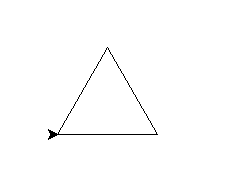
\includegraphics[width=2.0in]{img/triangle}
%    \vspace{-10mm}
    \end{center}
\end{ex}


\pagebreak
\section{Submitting}

You need to submit your code as a tarball (instructions below)
file. It should contain all files used in the exercises for this lab.
The submitted file should be named
\begin{center}
\texttt{cse107\_firstname\_lastname\_lab1.tar.gz}
\end{center}

Tar is used much the same way that Zip is used in Windows: it combines many
files and/or directories into a single file. Gzip is used in Linux to compress a
single file, so the combination of Tar and Gzip do what Zip does. However, Tar
deals with Gzip for you, so you will only need to learn and understand one
command for zipping and extracting.

In the terminal (ensure you are in your \texttt{lab1} directory), type the
following command, replacing \texttt{firstname} and \texttt{lastname} with your
first and last names:

\begin{bashcode}
$ tar czvf cse107_firstname_lastname_lab1.tar.gz *.py
\end{bashcode}

This creates the file \texttt{cse107\_firstname\_lastname\_lab1.tar.gz} in the
directory. The resulting archive, which includes every python file in your
\texttt{lab1} directory, is called a tarball. 

To check the contents of your tarball, run the following command:

\begin{bashcode}
$ tar tvf cse107_firstname_lastname_lab1.tar.gz
\end{bashcode}

You should see a list of your Python source code files.

\begin{center}
  \textbf{Upload your tarball to Canvas.}
\end{center}

\listoftheorems

\end{document}
